\documentclass[conference]{IEEEtran}
\usepackage{cite}
\usepackage{graphicx}
\usepackage{placeins}
\usepackage{float}
\usepackage{subfigure}
\begin{document}
\title{Projeto 1 de Introdu\c{c}\~ao ao Processamento de Imagens \\ Terceira Parte}
\author{\IEEEauthorblockN{Gabriel Martins de Miranda}
\IEEEauthorblockA{130111350\\
Universidade de Bras\'ilia\\
Email:gabrielmirandat@hotmail.com}
}
\maketitle
\begin{abstract}
Trabalho baseado nos templates IEEE.
\end{abstract}
\section{Resumo}
\label{sec:intro} 
O algoritmo apresentado neste relat\'orio apresenta um m\'etodo para, dada uma imagem bin\'aria (uma imagem que apresenta apenas dois n\'iveis de cinza, neste caso preto=0 e branco=255) contabilizar quantas manchas existem nela (conjunto de pixels pretos envoltos por pixels brancos ) e se existem buracos nestas manchas (conjunto de pixels brancos envoltos por pixels pretos). Foram utilizadas quatro imagens de teste, mostradas na se\c{c}\~ao $Resultados$.

\section{ Introdu\c{c}\~ao} 
\label{sec:meth} 
Algumas considera\c{c}\~oes inicias para o entendimento do leitor. Uma imagem pode ser vista como uma matriz, em que cada elemento recebe o nome de pixel e \'e a menor unidade da imagem. Se a imagem  n\~ao \'e colorida, como \'e o caso, ela \'e representada em n\'iveis de cinza, que v\~ao de $0$  a $ 2^n-1$, onde $n$ representa o n\'umero de bits que representam um pixel. O trabalho consiste em manipular estas representa\c{c}\~oes. A resolu\c{c}\~ao da imagem indica quantos pixels ela tem. No exemplo, $512$x$512$ = $[n\circ  de  linhas$ x $ n\circ  de  colunas]$ da matriz, totalizando em $262144$ pixels. 
 
\section{Metodologia} 
\label{sec:meth} 
Dada a imagem original, $p=p(x,y) $, foi criada uma nova imagem $f=f(x,y) $ com uma coluna a mais no extremo esquerdo e uma linha a mais na parte superior. Esta adapta\c{c}\~ao fez-se necess\'aria pois $\forall\;(x,y)\;\in Dom(p) $, foram comparados os pixels$(x-1,y) $ e $(x,y-1) $, sendo x o n\'umero de linhas e y o n\'umero de colunas. Criou-se uma matriz de r\'otulos, que chamaremos por $g=g(x,y) $, do mesmo tamanho de $f$, onde todo pixel branco $f(x,y)=255 $ foi mapeado para $g(x,y)=1$ e nenhuma mudan\c{c}a foi feita onde $f(x,y)=0$.

Percorreu-se $f $ pixel a pixel, e cada vez que $f(x,y)=0$ algumas compara\c{c}\~oes foram feitas, a saber:

Sendo $t=f(x-1,y )$, $r=f(x,y-1) $, $tr=g(x-1,y) $ e $rr=g(x,y-1)$
\begin{itemize}
	\item Se $ r==255 $ e  $t==255 $, $g(x,y)=novo\;rotulo$.
	\item Se $ r==0 $ e  $t==0 $ e $tr==rr$, $g(x,y)=tr$.
	\item  Se $ r==0 $ e  $t==0 $ e $tr\neq rr$,estabeleceu-se a equival\^encia entre $tr $ e $rr$,sendo  $\forall\;i\;\forall\;j\;\in [2 .. x]$x$[2 .. x] $, se $g(i,j)== max(tr,rr)\;\Rightarrow\;g(i,j)= min(tr,rr) $.
	\item A matriz de r\'otulos foi \''normalizada\'' para apresentar apenas valores de 2 a $N°\_de\_manchas +1$ para os pixels que representam as manchas.
	\item A rotula\c{c}\~ao das manchas foi similar a dos buracos.
\end{itemize}
\vspace{2\baselineskip}\vspace{-\parskip}
Fun\c{c}\~oes utilizadas:
\vspace{2\baselineskip}\vspace{-\parskip}
\begin{enumerate}
	 \item $preprocessamento.m$: Tem por objetivo binarizar a imagem original para que os pixels apresentem apenas $branco=255 $ e $ preto=0$.
  	\item $proc\_manchas.m$: mapear a matriz de r\'otulos das manchas. A fun\c{c}\~ao retorna a matriz de r\'otulos das manchas e um vetor\_linha cujos elementos representam os r\'otulos atribu\'idos as manchas e cujo $size $ \'e igual ao n\'umero de manchas.
  	\item $proc\_buracos.m$: mapear a matriz de r\'otulos dos buracos. Aqui a $f$ foi invertida, assim como a $g$ e o mesmo processo foi feito.
  	\item $juntador\_mancha\_buraco.m$ : Aqui foi criada uma nova matriz $z=z(x,y) $ dada por $z(x,y)=max(rotulos\_das\_manchas(x,y),rotulos\_dos\_buracos(x,y))$.
  	\item $detector.m$: realiza a quantifica\c{c}\~ao de buracos para cada mancha. Aqui foi utilizado o mesmo vetor de manchas criado anteriormente. Foi criada uma nova linha para o vetor, tornando-o uma matriz $[2 $x$n\circ de manchas]$. A cada verifica\c{c}\~ao de que um buraco pertence a uma mancha, sendo $(1,n) $ o \'indice da mancha,   $(2,n) $ \'e incrementado.
  	\item $resultado.m$: Mostra a interface com o usu\'uario, mostrando a sa\'ida gr\'afica na tela e os resultados na janela de comando.
  	
\end{enumerate}

\section{Resultados} 
\label{sec:meth} 
Sa\'idas gr\'aficas:
\begin{itemize}
  	\item Imagens analisadas:\\
		%\vspace{2\baselineskip}\vspace{-\parskip}
		\centering
\includegraphics[scale=0.5]{images/fig1}
		\centering
\includegraphics[scale=0.5]{images/fig2}
		\centering
\includegraphics[scale=0.5]{images/fig3}
		\centering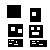
\includegraphics[scale=10.0]{images/fig4}
		\vspace{2\baselineskip}\vspace{-\parskip}

	\item Resultados da primeira imagem:
		\vspace{2\baselineskip}\vspace{-\parskip}
		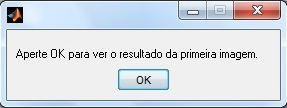
\includegraphics[scale=0.95]{images/janela1}
		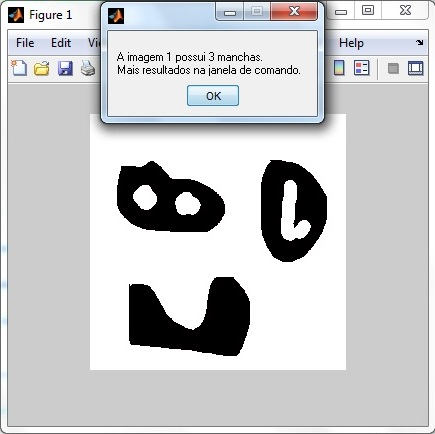
\includegraphics[scale=0.65]{images/janela1-2}
		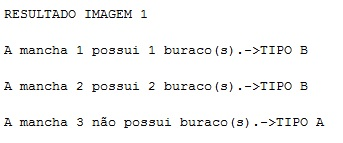
\includegraphics[scale=0.8]{images/comando1}
		\vspace{2\baselineskip}\vspace{-\parskip}
	\item Resultados da segunda imagem:
		\vspace{2\baselineskip}\vspace{-\parskip}
		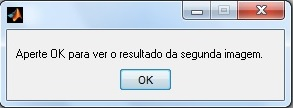
\includegraphics[scale=0.95]{images/janela2}
		\vspace{2\baselineskip}\vspace{-\parskip}
		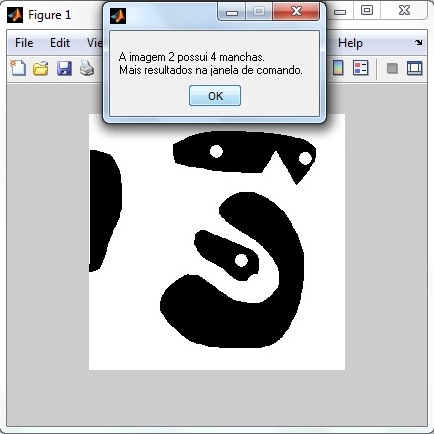
\includegraphics[scale=0.64]{images/janela2-2}
		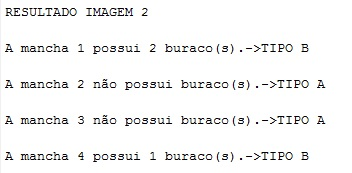
\includegraphics[scale=0.8]{images/comando2}
		\vspace{2\baselineskip}\vspace{-\parskip}

	\item Resultados da terceira imagem:
		\vspace{2\baselineskip}\vspace{-\parskip}
		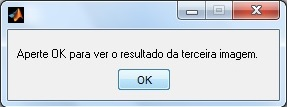
\includegraphics[scale=0.95]{images/janela3}
		\vspace{2\baselineskip}\vspace{-\parskip}
		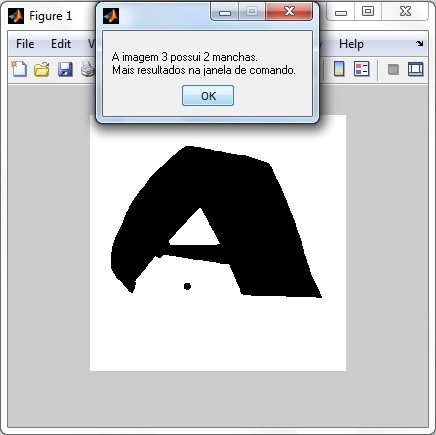
\includegraphics[scale=0.65]{images/janela3-2}
		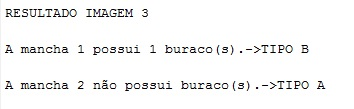
\includegraphics[scale=0.8]{images/comando3}
		\vspace{2\baselineskip}\vspace{-\parskip}
	
	\item Resultados da quarta imagem:
		\vspace{2\baselineskip}\vspace{-\parskip}
		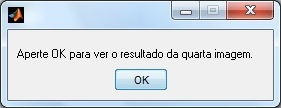
\includegraphics[scale=0.95]{images/janela4}
		\vspace{2\baselineskip}\vspace{-\parskip}
		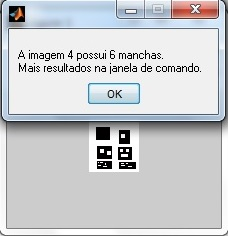
\includegraphics[scale=1.0]{images/janela4-2}
		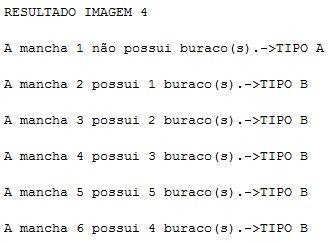
\includegraphics[scale=0.8]{images/comando4}
		\vspace{2\baselineskip}\vspace{-\parskip}

 \end{itemize}

\section{Conclus\~ao} 
\label{sec:meth} 

Foi poss\'ivel observar a import\^ancia de algoritmos de detec\c{c}\~ao de padr\~oes em imagens, que podem ser usados em diversas \'areas, como por exemplo na \'area de sa\'ude.

\end{document}